\documentclass[10pt,a4paper,titlepage]{article}
\usepackage{latexsym}
\usepackage[a4paper,top=2.5cm,bottom=2.5cm,left=2.5cm,right=2.5cm]{geometry}
\usepackage[utf8x]{inputenc}
\usepackage{booktabs,caption,amsfonts,amssymb,fancyhdr, amsmath}
\usepackage[english]{babel}
\usepackage{indentfirst}
\usepackage{multirow}
\usepackage{float}
\renewcommand*{\familydefault}{\sfdefault}
\usepackage{graphicx}
\usepackage{yfonts}
\usepackage{mathrsfs}
\usepackage{hyperref}
\usepackage{color}
\usepackage{subcaption}
\usepackage{listings}


\lstset{language=c++}
\lstset{backgroundcolor=\color{white}}
\lstset{frame=single}
\lstset{stringstyle=\ttfamily}
\lstset{keywordstyle=\color{red}\bfseries}
\lstset{commentstyle=\itshape\color{blue}}

%\captionsetup[table]{position=top}
\addtolength{\textwidth}{1cm}
\addtolength{\hoffset}{-1cm}
\pagestyle{headings}
\begin{document}
\begin{center}
{\LARGE \bfseries Computational Physics\par}
\vspace{0.5cm}
{\LARGE \bfseries Project 4 \par}
\vspace{0.5cm}
{\bfseries \today \par}
\end{center}

\vspace{1cm}

\begin{tabular*}{\textwidth}{@{}l@{\extracolsep{\fill}}l@{}}
Academic year 2015-2016	 &Team group: \\
						&Giulio Isacchini\\
                        &Giovanni Pederiva\\
                        &Alessio Pizzini\\
                        &Mattia Ubertini\\
                                           
\end{tabular*}
\begin{center}
\hrule height 2 pt
\end{center} 
\section*{Abstract}
\noindent The aim of this project is to implement the Ising model for a 2 dimensional squared lattice. This model describes a magnetic material that we simplify by considering a system composed of particles,  that we assume to be fixed in a lattice, which can have either spin up or down and react to the interaction with each other by changing their spin. \\
The Metropolis algorithm has been applied to compute the probability rates of transitions during the Monte Carlo simulations. Thermodynamical parameters such as the energy $E$, the mean magnetization $\mathscr{M}$, the specific heat $C_{V}$ and the susceptibility $\chi$ have been studied as functions of the temperature $T$ around its critical value $T_C$ (viz. Curie temperature).
\section*{Analysis of the problem}
\noindent The Ising model allows us to describe in a simple way the behavior of a magnetic material depending on its thermal energy and an external magnetic field. We will now assume that our lattice is made by a squared grid of atoms, which spin can be either -1 or +1. \\ 
In its simplest form, the Ising model approximates the energy given by the interaction of the magnetic spins as 
\begin{equation}
E= -J \sum_{<kl>}^{N}s_{k}s_{l}- 
\mathscr{B} 
\sum_{k}^{N}s_{k}
\end{equation}
where $J$ is a constant expressing the strength of the interaction between spins and the notation $<kl>$ means that the sum has to be computed on neighboring particles only. In our case, there is no external magnetic field $\mathscr{B}$, so the second term vanishes. \\
We will later have to compare the results provided by this algorithm with the expectation value of these quantities. To calculate them, we can exploit our knowledge about the energies: 
\begin{equation}
P_{i}(\beta)=\frac{e^{-\beta E_{i}}}{Z}
\end{equation}
being $\beta = \frac{1}{k_{b}T}$, $k_{b}$ the Boltzmann constant, $E_{i}$ the energy of the state $i$, $Z$ the partition function of the canonical ensamble 
\begin{equation}
Z = \sum_{i=1}^{M}e^{-\beta E_{i}}
\end{equation}
where the index $i$ labels every possible microstate.\\
The other thermodynamical parameters are defined as follows:
\begin{equation}
\mathscr{M} = \sum_{j=1}^{N}s_{j}
\end{equation}
\begin{equation}
C_{V}=\frac{1}{k_{b}T^{2}}\big( \langle E^{2} \rangle - \langle E \rangle ^{2} \big)
\end{equation}
\begin{equation}
\chi = \frac{1}{k_{b}T} \big( \langle \mathscr{M}^{2} \rangle - \langle \mathscr{|M|} \rangle ^{2} \big)
\end{equation}
As previously stated, we used the Metropolis algorithm to simulate spin flipping. It works as follows: 
\begin{itemize}
\item start with an initial configuration, which could be either a random one or a all-up one (we have ran our algorithm in both cases) and compute the energy of the whole system
\item pick a random position in the spin matrix and compute the energy of the lattice after having flipped the chosen spin
\item now compare the energy of the system before and after the flip; if it has decreased, accept the move, otherwise accept it with a probability of $e^{-\beta \Delta E}$, where $\Delta E$ is the difference of the two energies and $\beta$ is $\frac{1}{kT}$
\item the final configuration is now the initial one to start with
\end{itemize}
We have implemented this algorithm for different values of temperature between $\frac{k_{b}T}{J} = 1$ and $\frac{k_{b}T}{J} = 2.4$ and for different sizes of the lattice from a $2\times 2$ one (for which the expected theoretical values are rather simple to compute) to a $200\times 200$ one. Periodic boundary conditions have been applied.\\
The Ising model undergoes a phase transition of second order, i.e. below a critical temperature $T_{C}$ (Curie temperature) the system has a spontaneous magnetization, being $\langle \mathscr{M}\rangle \neq 0$, while above $T_{C}$ $\langle \mathscr{M}\rangle = 0$. $\langle \mathscr{M}\rangle$ is normally called the order parameter. 
\\An analytic expression for $|\mathscr{M}|$ can be derived assuming the probability distribution for the states (2) and periodic boundary conditions, resulting in the following formulas (Onsager, 1944):
\begin{equation}\begin{split}
|\mathscr{M}|=&\bigg[1-\frac{(1-tanh^{2}(\beta J))^{4}}{16tanh^{4}(\beta J)}\bigg]^{\frac{1}{8}}~~ \mbox{for}~~~ \ T<T_{C}\\
|\mathscr{M}|=&\ 0 \ ~~~~~~~~~~~~~~~~~~~~~~~~~~~~~~~~ \mbox{for}~~~ \ T \ > \ T_{C}
\end{split}\end{equation}
So, we expect a sharp decrease in the absolute value of the average magnetization around $T_{C}$.
Onsager's calculations also gave the following relation for the specific heat:
\begin{equation}
C_{V} \sim -\frac{2}{\pi} \bigg(\frac{2J}{k_{b}T_{C}}\bigg) ln \Bigg|1-\frac{T}{T_{C}} \Bigg| + const
\end{equation}
The two previous result are a special case of the general power law derived by critical phenomena theories, which holds for $T < T_{C}$: 
\begin{equation}\begin{split}
\langle \mathscr{M}(T)\rangle &\sim (T-T_{C})^{\beta}\\
C_{V} &\sim | T_{C} - T |^{-\alpha}
\end{split}\end{equation}
where $\beta = \frac{1}{8}$ is the so called critical exponent and $\alpha \rightarrow$ 0, so also $C_{V}$ is expected to have a sharp peak around $T_{C}$.\\
The susceptibility $\chi$ is also expected to have a peak in its critical region. Theories of critical phenomena lead to:
\begin{equation}
\chi(T) \sim |T_{C}-T|^{-\frac{7}{4}}
\end{equation}
Calculations made by Onsager also provided with an expected value for the critical temperature:
\begin{equation}
\frac{k_{b}T_{C}}{J}=\frac{2}{ln(1+\sqrt{2})} \simeq 2.269
\end{equation}
while the estimate of the critical temperature from a matrix having dimension N can be derived from the so-called finite size scaling relations, resulting in:
\begin{equation}
T_{C}(L)-T_{C}(L \rightarrow \infty) = aL^{-\frac{1}{\nu}}
\end{equation}
Merging the last equation with (9) and (10), we get:
\begin{equation}\begin{split}
\langle \mathscr{M}(T)\rangle &\rightarrow L^{-\frac{\beta}{\nu}}\\
C_{V}(T) &\rightarrow L^{\frac{\alpha}{\nu}}\\
\chi (T) &\rightarrow L^{\frac{\gamma}{\nu}}
\end{split}\end{equation}
which hold when T is approaching $T_{C}$.
\section*{2 x 2 Case} 
\noindent First we have studied the most simple case. A system represented by a $2 \times 2 $ lattice. We have studied it analytically and then we have used the derived results as benchmark to test our implemented Metropolis algorithm.
\\ 
We have analytically computed the quantities, which characterized the system: 
\begin{itemize}
\item The expectation values of the energy of the system $\langle E \rangle$
\item  The expectation values of the absolute value of magnetization $\langle |M| \rangle$
\item The variance of the energy $\sigma ^2_E= (\langle E^2\rangle-\langle E \rangle ^2)$
\item The variance of the absolute value of the magnetization $\sigma^2_{|M|}= (\langle |M|^2\rangle-\langle |M| \rangle ^2)$
\end{itemize}
In particular through the last two parameters we have been able to derive also the heat capacity and susceptibility of the system. 
\\
All these terms depend on the temperature. At the beginning we have derived the general relations for all of them, then we have calculated the values for $k_b T/ J=1$.
In the next calculation we have set the constant of coupling $J=1$. \\
The possible configurations of the system are $2^4$. 
First we have focused on the partition function $Z$; in this case there actually are just three different possible value of energy for the different configurations. 
There are two configurations with $E=-8J$ which correspond to the configurations with all the spin aligned in both the directions. There are two configurations with $E=8J$ corresponding to the configurations with the aligned spin in the two diagonals. All the others twelve configurations have $E=0J$.
This means that $$Z=2 e^{ 8 \beta }+2e^{- 8 \beta }+12$$
\\
Then exploiting the relations shown before we see that the expectation values of $E$, as the other parameters, just depend on the configuration $i$ with $E_i \neq 0$. 
This means that we have just four contributing configurations.  Two different configurations with $E_i=-8J$ and other two different configurations with $E_i= 8J$. This leads us to the expression for its expectation value:  
\begin{equation}
\langle E \rangle=\frac{2 \times -8 e^{8 \beta}+2 \times 8 e^{-8 \beta} }{2 e^{ 8 \beta }+2e^{- 8 \beta }+12}
\end{equation}
Then for the expectation value of $|M|$:  we have one configuration with $M=4$ and another one with $M=-4$ corresponding to the lattice with all spins aligned in the same direction, all up or all down. Both these configurations have $E_i=-8J$. Then we have four configurations with $M=2$ and four with $M=-2$ corresponding to the lattices with $3$ spin aligned in one direction and just one in the opposite one. In this case all these configurations have $E_i=0J$. All the other six configurations have $M=0$.
\\
Since we are considering the expectation value of the absolute value $|M|$, the configurations with opposite  $M$ have to be put together. This means that $\langle |M| \rangle$ reads: 
\begin{equation}
\langle |M| \rangle=\frac{2 \times 4 e^{8 \beta}+8 \times 2}{2 e^{ 8 \beta }+2e^{- 8 \beta }+12}
\end{equation}
\\
For the variance of $E$ we need first to derive the expectation value $\langle E^2 \rangle$. In this case we have two configurations with $E^2=64 J^2$ with $E_i=-8J$ and other two with the same $E^2=64J^2$ but with $E_i=8 J$. So we can finally write the expectation value: 
\begin{equation}
\langle E^2 \rangle = \frac{2 \times 64 e^{8 \beta}+2 \times 64 e ^{-8 \beta}}{2 e^{ 8 \beta }+2e^{- 8 \beta }+12}
\end{equation}
At this point we can finally derive the expression for the variance $\sigma^2_E=(\langle E^2\rangle-\langle E \rangle ^2)$:
\begin{center}
\begin{equation}\sigma^2_E=\frac{2 \times 64 e^{8 \beta}+2 \times 64 e ^{-8 \beta}}{2 e^{ 8 \beta }+2e^{- 8 \beta }+12}-\left(\frac{2 \times -8 e^{8 \beta}+2 \times 8 e^{-8 \beta} }{2 e^{ 8 \beta }+2e^{- 8 \beta }+12}\right)^2
\end{equation}
\end{center}
Then the heat capacity is related to the variance through the relation: $$C_v=\frac{\sigma^2_E}{k_b T^2}$$
\newpage
\noindent Finally for the variance $\sigma^2_{|M|}$ first we need  first to derive the expression for $\langle |M|^2 \rangle$. In this $2 \times 2$ lattice as shown before there are just two configurations with $|M|=4$ and energy $E_i=-8J$ and other $8$ configurations with $|M|=2$ and energy $E_i=0J$. These simply lead us to the expression: 
\begin{equation}
\langle|M|^2\rangle=\frac{2 \times 16 e ^{8 \beta}+ 8 \times 4}{2 e^{ 8 \beta }+2e^{- 8 \beta }+12}
\end{equation}
So the expression for the variance reads: \begin{center}
\begin{equation}\sigma^2_{|M|}=\frac{2 \times 16 e ^{8 \beta}+ 8 \times 4}{2 e^{ 8 \beta }+2e^{- 8 \beta }+12}-\left(\frac{2 \times 4 e^{8 \beta}+8 \times 2}{2 e^{ 8 \beta }+2e^{- 8 \beta }+12}\right)^2
\end{equation}
\end{center}
The susceptibility is related to the variance through: $$\chi=\frac{\sigma^2_{|M|}}{k_b T}$$
So once we have derived these relations we have been able to compute from them these quantities and then we have compared them with the same ones got through our algorithm. We have done the comparison in the case with $k_b T=1$
\\
We have collected some data got through our Metropolis algorithm with different number of Monte Carlo cycles. 
For each number of Monte Carlo cycles we have performed a loop collecting data 1000 times and then we have averaged the data collected. We have done these with an initial random lattice and also starting from a lattice with all spin aligned. 
\\
Here we present the data obtained and comparing them with the values got analytically:
\\
\begin{minipage}[b]{0.5\textwidth}\centering
\begin{table}[H]
\caption{{\footnotesize Analytic value for  $\langle E \rangle = -7.9839 ~ J$}}
\begin{center}

\begin{tabular}[t]{|p{2.3cm}|p{2.3cm}|p{2.3cm}|}
\hline
N. of Monte Carlo cycles & $\langle E/J \rangle$   with up matrix & $\langle  E/J \rangle $   with random matrix \\\hline
$10^{1}$ & -8 &-7.2\\\hline
$10^{2}$& -8 &-7.68\\\hline
$10^{3}$ &  -7.96 &-7.984\\\hline
$10^{4}$ & -7.988 &-7.9816\\\hline
$10^{5}$& -7.9816 &-7.98544\\\hline
$10^{6}$& -7.98342 &-7.9851\\\hline

\end{tabular}
\end{center}
\end{table}
\end{minipage}
\begin{minipage}[b]{0.5\linewidth}\centering
\begin{table}[H]
\caption{{\footnotesize Analytic value for  $\sigma^{2}(E)  = 0.1282 J^2$}}
\begin{center}
\begin{tabular}[t]{|p{2.3cm}|p{2.3cm}|p{2.3cm}|}
\hline
N. of Monte Carlo cycles & $ \sigma^{2}(E)/J^2$  with up matrix & $ \sigma^{2}(E)/J^2$   with random matrix \\\hline
$10^{1}$ & 0 &5.76\\\hline
$10^{2}$& 0 &2.4576\\\hline
$10^{3}$ &  0.3184 &0.127744\\\hline
$10^{4}$ & 0.095856 &0.146861\\\hline
$10^{5}$& 0.146861 &0.116268\\\hline
$10^{6}$& 0.132397 &0.118946\\\hline
\end{tabular}
\end{center}
\end{table}
\end{minipage}


\noindent We notice that our estimates for $\langle E \rangle$ with 100 Monte Carlo cycles or more are compatible with the analytic value, since the difference between the former and the latter is about or less than $\sigma(E)$. For a smaller number of Monte Carlo cycles, instead, the system hasn't reached its steady state yet and is still in its initial state, since the probability for a flip to happen is very small in this case ($K_{b}T=1$). The estimate made with $10^6$ Monte Carlo cycles provides us with a value having 4 exact leading digits starting from an "up" configuration and 3 exact leading digits starting from a random matrix. As for the $\sigma^{2}(E)$, our estimates agree with its analytic value only up to the first leading digit even with $10^6$ Monte Carlo cycles, even if this precision can be already achieved with  1000 cycles if we start with a random initial configuration.
\\
\begin{minipage}[b]{0.5\textwidth}\centering
\begin{table}[H]
\caption{{\footnotesize Analytic value for  $\langle |\mathscr{M}| \rangle$ = 3.9946}}
\begin{center}
\begin{tabular}[t]{|p{2.3cm}|p{2.3cm}|p{2.3cm}|}
\hline
N. of Monte Carlo cycles & $\langle |\mathscr{M}| \rangle$  with up matrix & $\langle  |\mathscr{M}| \rangle $  with random matrix \\\hline
$10^1$ & 4 & 3.8\\\hline
$10^2$& 4 &3.88\\\hline
$10^3$ &  3.986 &3.9944\\\hline
$10^4$ & 3.996 &3.9958\\\hline
$10^5$& 3.99392 &3.99518  \\\hline
$10^6$& 3.99451 &3.99501\\\hline
\end{tabular}
\end{center}
\end{table}
\end{minipage}
\begin{minipage}[b]{0.5\linewidth}\centering
\begin{table}[H]
\caption{{\footnotesize Analytic value for  $\sigma^2_{|\mathscr{M}|}$ = 0.0160}}
\begin{center}
\begin{tabular}[t]{|p{2.3cm}|p{2.3cm}|p{2.3cm}|}
\hline
N. of Monte Carlo cycles & $ \sigma^2_{|\mathscr{M}|}$  with up matrix & $\sigma^2_{|\mathscr{M}|}$  with random matrix \\\hline
$10^1$ & 0 & 0.36\\\hline
$10^2$& 0& 0.3856\\\hline
$10^3$ &  0.04384 &0.019964\\\hline
$10^4$ & 0.011984 &0.017564\\\hline
$10^5$& 0.018043 &  0.0143368  \\\hline
$10^6$& 0.016313 &0.0150191\\\hline
\end{tabular}
\end{center}
\end{table}
\end{minipage}


\noindent As in the previous case, our estimates for $\langle|\mathscr{M}|\rangle$ differ from its analytic value for about or less than $\sigma_{|\mathscr{M}|}$ for 100 or more Monte Carlo cycles, but only with $10^6$ cycles we can achieve an estimate having 4 correct leading digits, if we start with an up matrix, while we have only 3 correct leading digits starting with a random configuration. As for the variance $\sigma^{2}_{|\mathscr{M}|}$, with $10^6$ Monte Carlo cycles we have two correct leading digits starting from a up matrix and only one with a random one.
\\The computed variance of the absolute magnetization, as it was for the variance of the energy,  $|\mathscr{M}|$ has resulted to be much less reliable than its own value. 
\\
We have compared the variance for both the quantities, the same considerations hold for the comparison of heat capacity and the susceptibility since these quantities are proportional to the variances through some constants, because in all this case $T$ is fixed. 

\section*{Study of transitory states and equilibrium, 20 x 20 case}
\noindent We choose now a square matrix having size equal to $L=20$ spins. We want to analyze how much time (number of MC cycle) one needs in order to reach an equilibrium position and start computing some expectation values of the system. The steps for doing this are the following.

\noindent Firstly we set $T=1$ and all the spin of the matrix pointing upwards. Then we make the calculation of Energy and Absolute Magnetization as a function of Monte Carlo cycles.
In the next step we perform the same experiment a great number of times (in our case around $10^4$ times for both Energy and Absolute Magnetization) and take the mean value of these quantities for every number of cycle.
Lastly we repeated the same process setting $T=2.4$ and using a random-spin-matrix.

\noindent Given the great number of operations a parallelization of the code with MPI was needed. In our case before the parallelization  it took around 15 minutes for creating two plots, afterwards around 5 minutes.
Here we show the results of the analysis.
\begin{figure}[H]
\begin{subfigure}{.5\textwidth}
  \centering
  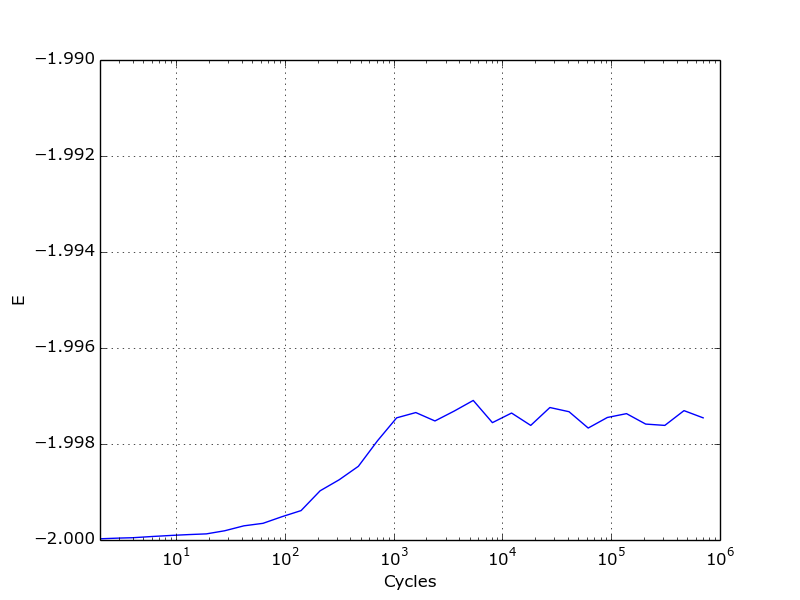
\includegraphics[width=.8\linewidth]{ENERGY_T1_UP_10000MEAN}
  \caption{{\footnotesize Average Energy - Up matrix}}
  \label{fig:sfig1}
\end{subfigure}%
\begin{subfigure}{.5\textwidth}
  \centering
  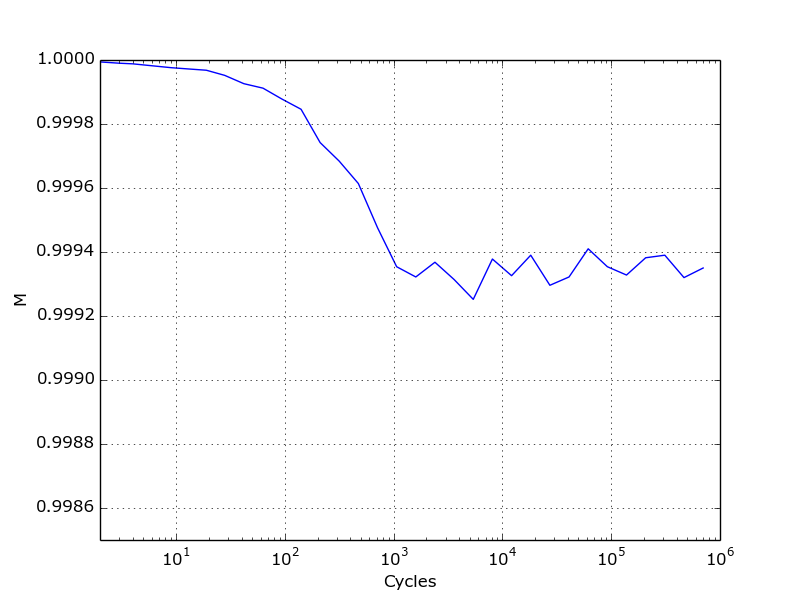
\includegraphics[width=.8\linewidth]{MAGNETIZATION_T1_UP_10000MEAN}
  \caption{{\footnotesize Average Magnetization - Up Matrix}}
  \label{fig:sfig2}
\end{subfigure}
\begin{subfigure}{.5\textwidth}
  \centering
  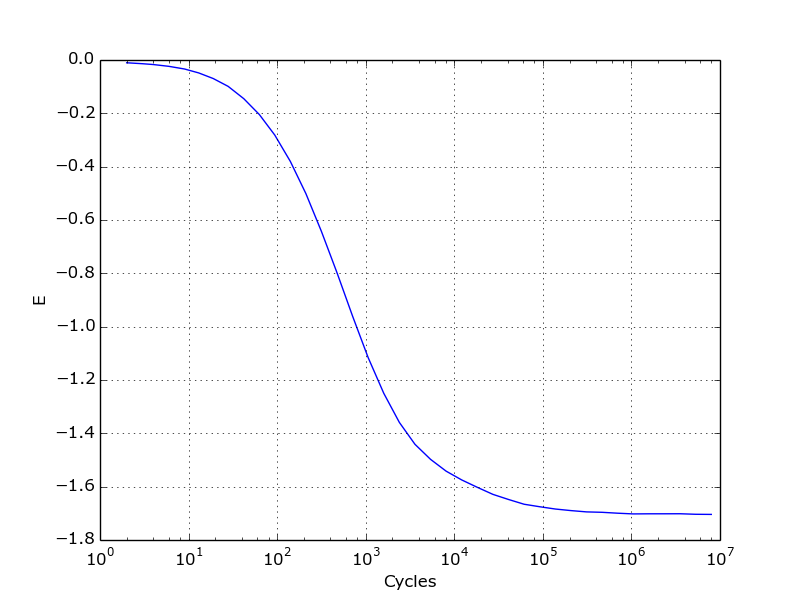
\includegraphics[width=.8\linewidth]{ENERGY_T1_RAND_1000MEAN}
  \caption{{\footnotesize Average Energy - random matrix}}
  \label{fig:sfig2}
\end{subfigure}
\begin{subfigure}{.5\textwidth}
  \centering
  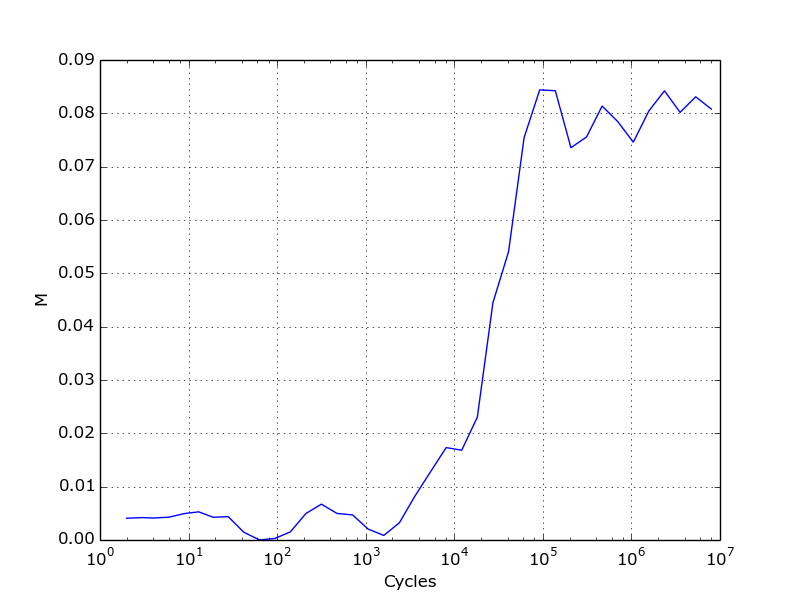
\includegraphics[width=.8\linewidth]{MAGNETIZATION_T1_RAND_1000MEAN}
  \caption{{\footnotesize Average Magnetization - Random Matrix}}
  \label{fig:sfig2}
\end{subfigure}
\caption{{\footnotesize The first four plots are made at $T=1$. In the plots $(a)$ and $(b)$, made with the up-spin-matrix, is clear that after $10^4$ cycles the values start to oscillate around an equilibrium position. On the other hand, for plots  $(c)$ and $(d)$ made with the random-spin-matrices, given the low temperature, it takes a lot more time and the values reach the equilibrium position around $10^6$ cycles.}}
\label{fig:fig}
\end{figure}
\begin{figure}[H]
  \centering
\begin{subfigure}{.42\textwidth}
  \centering
  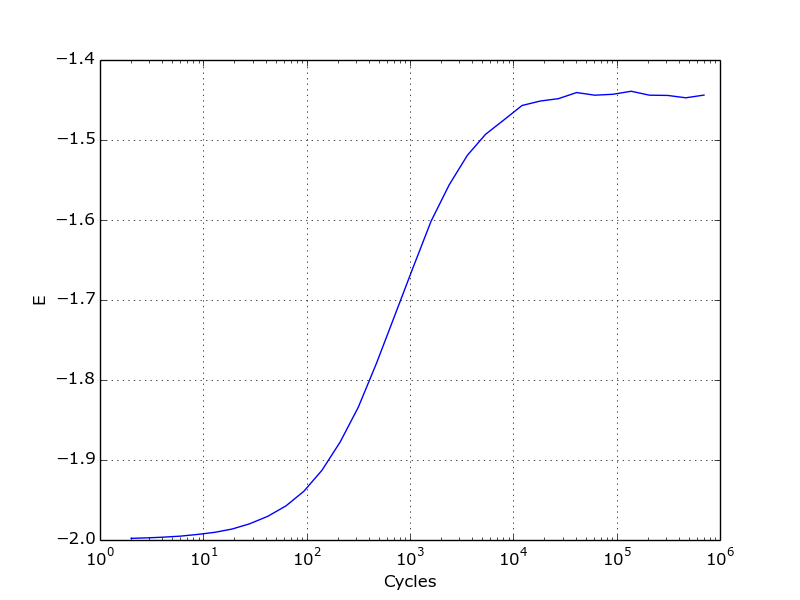
\includegraphics[width=.8\linewidth]{ENERGY_T24_UP_10000MEAN}
  \caption{{\footnotesize Average Energy - Up matrix}}
  \label{fig:sfig1}
\end{subfigure}%
\begin{subfigure}{.42\textwidth}
  \centering
  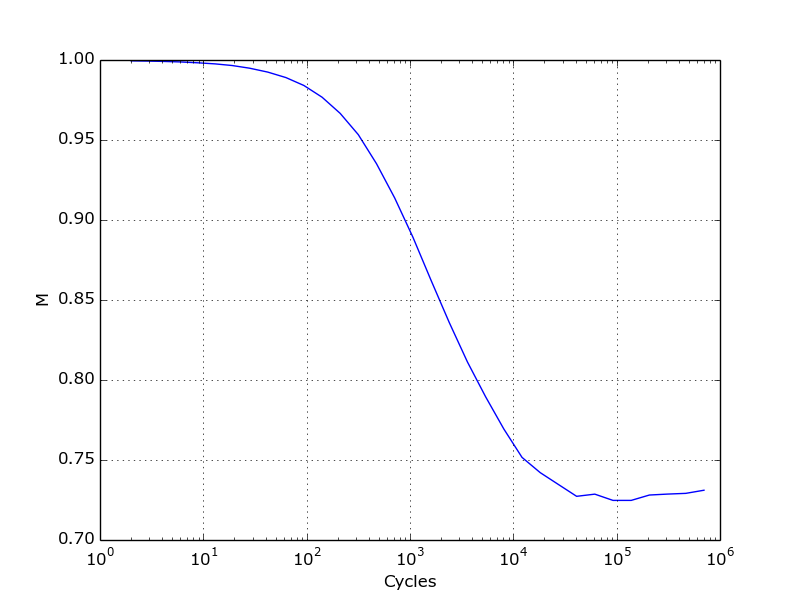
\includegraphics[width=.8\linewidth]{MAGNETIZATION_T24_UP_10000MEAN}
  \caption{{\footnotesize Average Magnetization - Up Matrix}}
  \label{fig:sfig2}
\end{subfigure}
\begin{subfigure}{.42\textwidth}
  \centering
  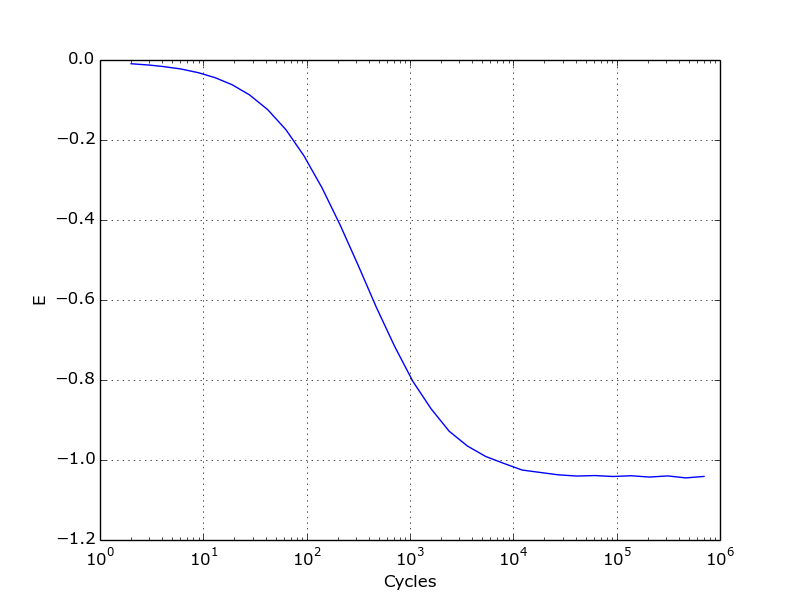
\includegraphics[width=.8\linewidth]{ENERGY_T24_RAND_10000MEAN}
  \caption{{\footnotesize Average Energy - Random matrix}}
  \label{fig:sfig2}
\end{subfigure}
\begin{subfigure}{.42\textwidth}
  \centering
  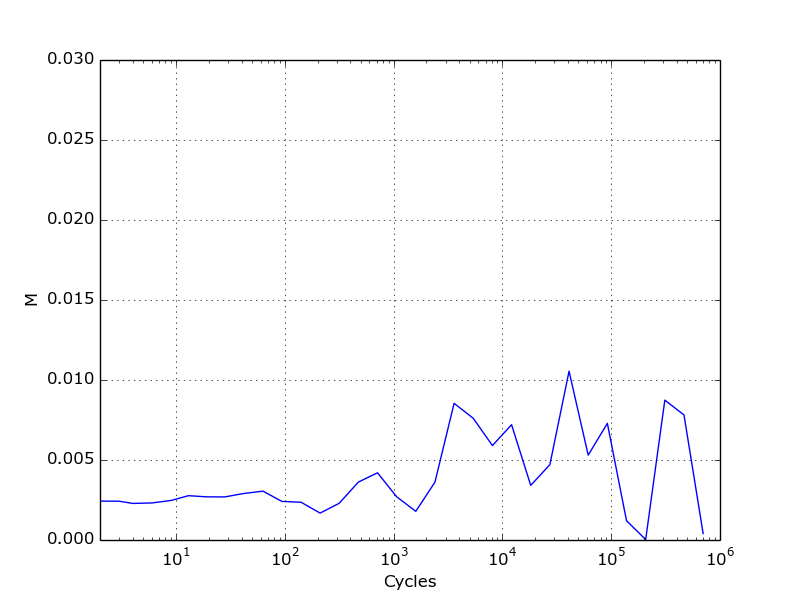
\includegraphics[width=.8\linewidth]{MAGNETIZATION_T2_RAND_10000MEAN}
  \caption{{\footnotesize Average Magnetization - Random Matrix}}
  \label{fig:sfig2}
\end{subfigure}
\caption{{\footnotesize These four plots are made at $T=2.4$.In the plots $(a)$ and $(b)$, made with the up-spin-matrix, the values reach the equilibrium after $10^5$ cycles Also for for plots  $(c)$ and $(d)$ made with the random-spin-matrices, given the high temperature and the fact that we start at random spin values, it takes a shorter time compared to $T=1$ and the values reach the equilibrium position around $10^5$ cycles.}}
\label{fig:fig}
\end{figure}
\noindent In conclusion the analysis tell us that after $10^6$ cycles we are sure to be in the equilibrium regime and that's were we can start to compute average values of the quantities we are interested to. We can generalize this approach by dividing this value for the size of the matrix.
As a result we can state that for a general $L\times L$ spin-Matrix, it's safe to start averaging after $N_{start}$ cycles with:
\begin{equation}
N_{start}=10^4\times L^2
\end{equation}
\noindent A closer look at the dependency of the probability of a spin flip as a function of temperature is needed in order to explain the phenomena just analyzed. Qualitatively, since the metropolis algorithm is based on the comparison between a random number and the factor $e^{- \frac{\Delta E}{T}}$, the number of accepted points will grow with the temperature and will be generally higher for the starting up-spin-matrix than the starting random-spin-matrix. A quantitative analysis is here shown.  \\ 
\begin{figure}[H]
\centering
\begin{subfigure}{.42\textwidth}
  \centering
  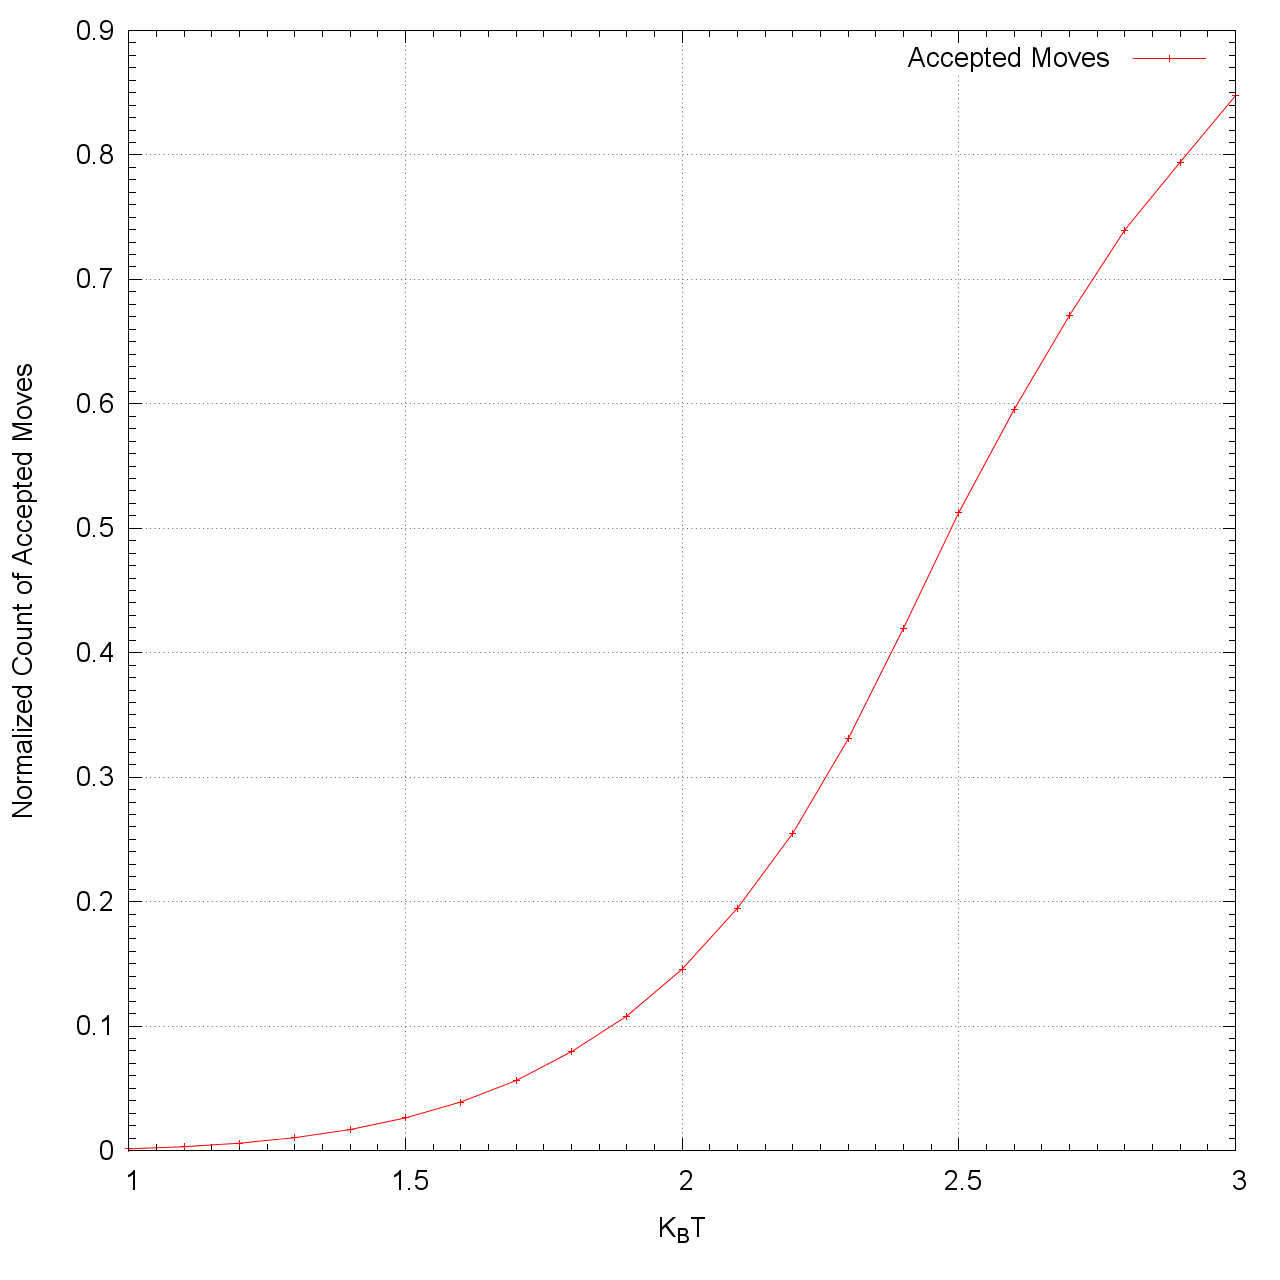
\includegraphics[width=.8\linewidth]{Flip_Counts_Up}
  \caption{{\footnotesize Up initial configuration}}
  \label{fig:sfig1}
\end{subfigure}%
\begin{subfigure}{.42\textwidth}
  \centering
  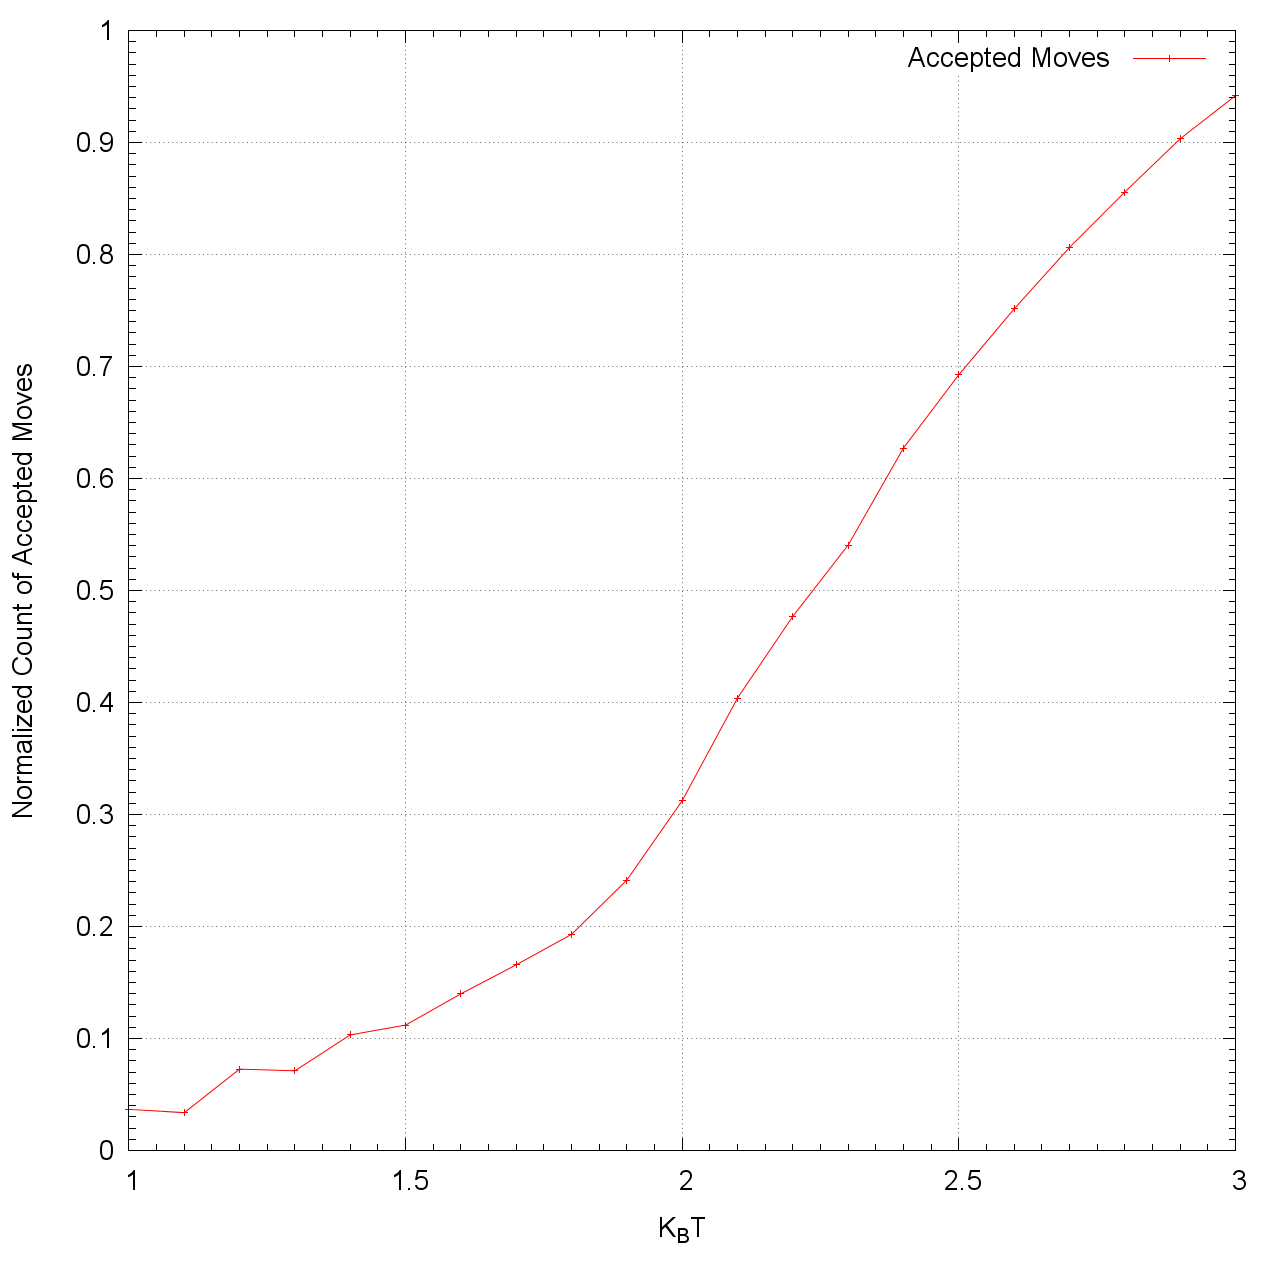
\includegraphics[width=.8\linewidth]{Flip_Counts_Rand}
  \caption{{\footnotesize Random initial configuration}}
  \label{fig:sfig2}
\end{subfigure}
\caption{{\footnotesize Number of spin flip as a function of the temperature. As expected the random initial configuration leads to a greater number of spin flips, and the function increase also with the temperature.}}
\label{fig:fig}
\end{figure}
\paragraph{Computation of P(E)}We have studied in more depth the lattice system $20 \times 20$ and we have managed to compute the probability for the system to be in a configuration with a certain energy. 
\\We point out that this probability does not distinguish the different configurations with the same energy. We have used the implemented Metropolis algorithm, in which we made the program count how many times the system turned in a configuration with a certain energy $E_i$.  As output we had two arrays, one with the stored energies, which the system assumed, and the other one the number of times those energies were measured.
\\ At this point the probability of a certain energy $E_i$ is represented by the number of times it was measured normalized with the total number of measurements: $$P(E_i)= \frac{N_i}{\sum_{i} N_i}$$
being $N_{i}$ the number of counts of configurations having energy equal to $E_{}$.
\\Once got the $P(E_i)$,exploiting it, we have computed the expectation value of $E$ and its variance. This way,with which we have computed these parameters, is equal, also mathematically, to the one used in the metropolis algorithm. The expectation value is computed in this case as: $\langle E \rangle = \frac{\sum_{i}N_i E_i}{\sum_{i}N_i}$, in the metropolis algorithm is computed by simply averaging all the terms: $\langle E \rangle = \frac{\sum_{i}E_i}{N_i}$ but obviously the last expression can be rewritten as the first one. This explanation still holds for the variance.  For this reason we haven't compared the results got in this way with the others. This doesn't imply that the results are exactly the same, because they   are all affected by random fluctuations. 
\\
We have computed the probability $P(E)$ for many different temperatures starting in both configurations of spin aligned and randomly distributed.
\\ 
\begin{center}
\begin{figure}[H]
 \centering
\begin{subfigure}{.5\textwidth}
  \centering
  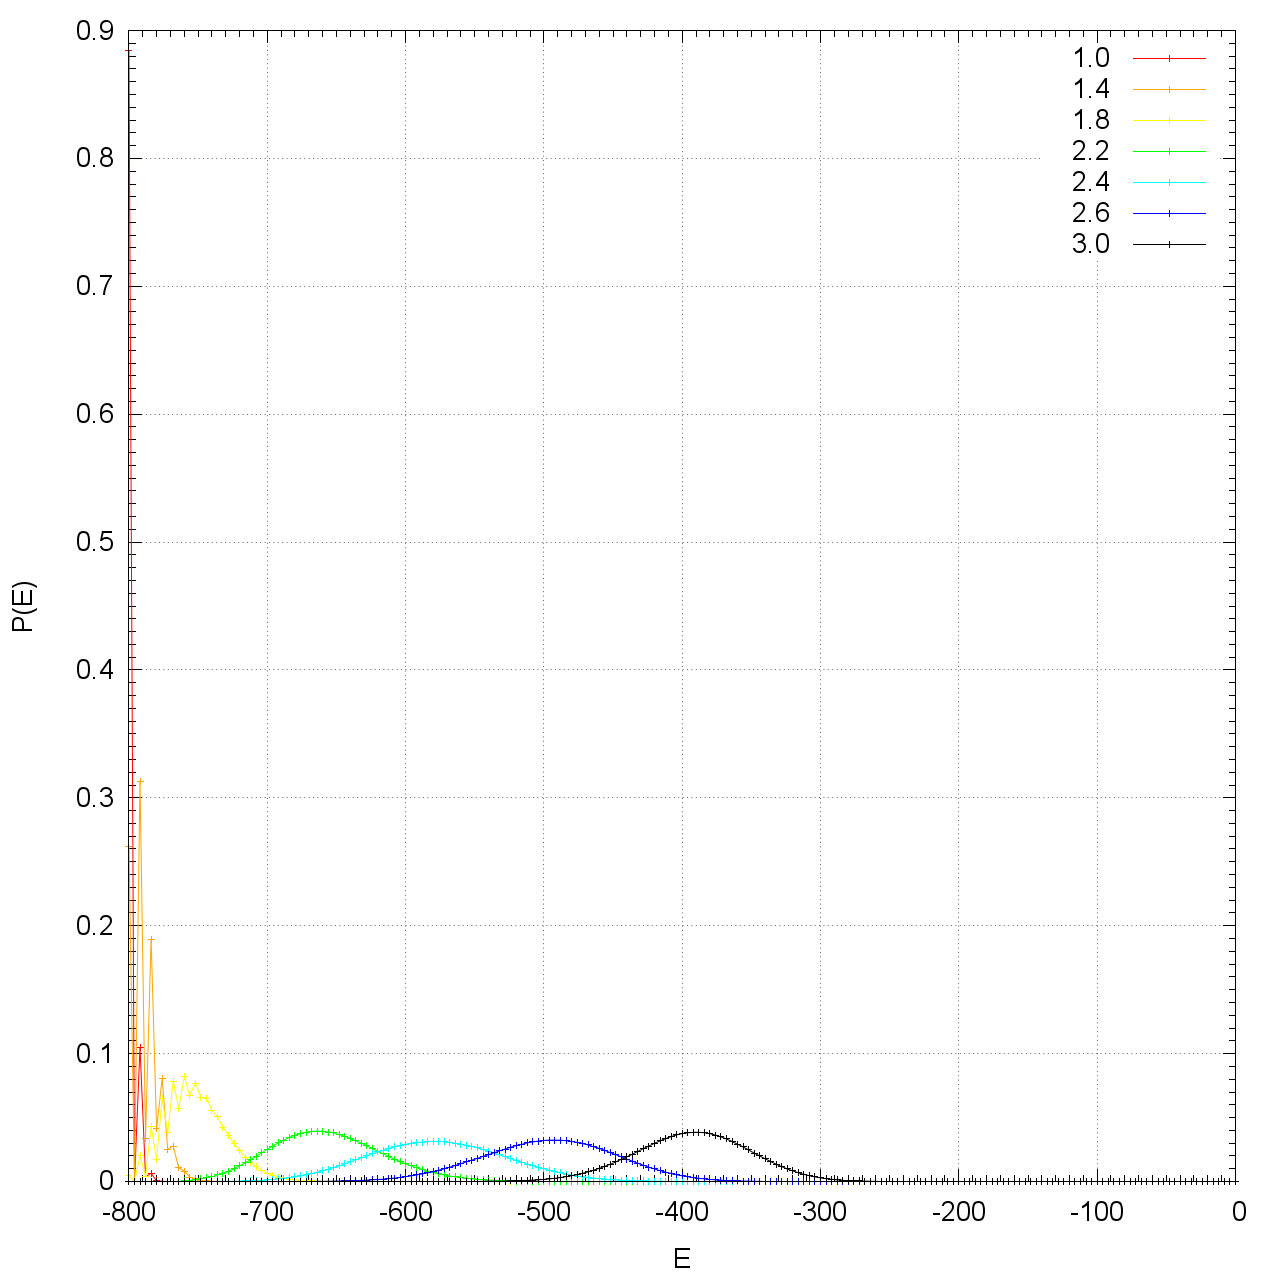
\includegraphics[width=.8\linewidth]{Energy_Counts}
  \caption{{\footnotesize Up initial configuration}}
  \label{fig:sfig1}
\end{subfigure}%
\begin{subfigure}{.5\textwidth}
  \centering
  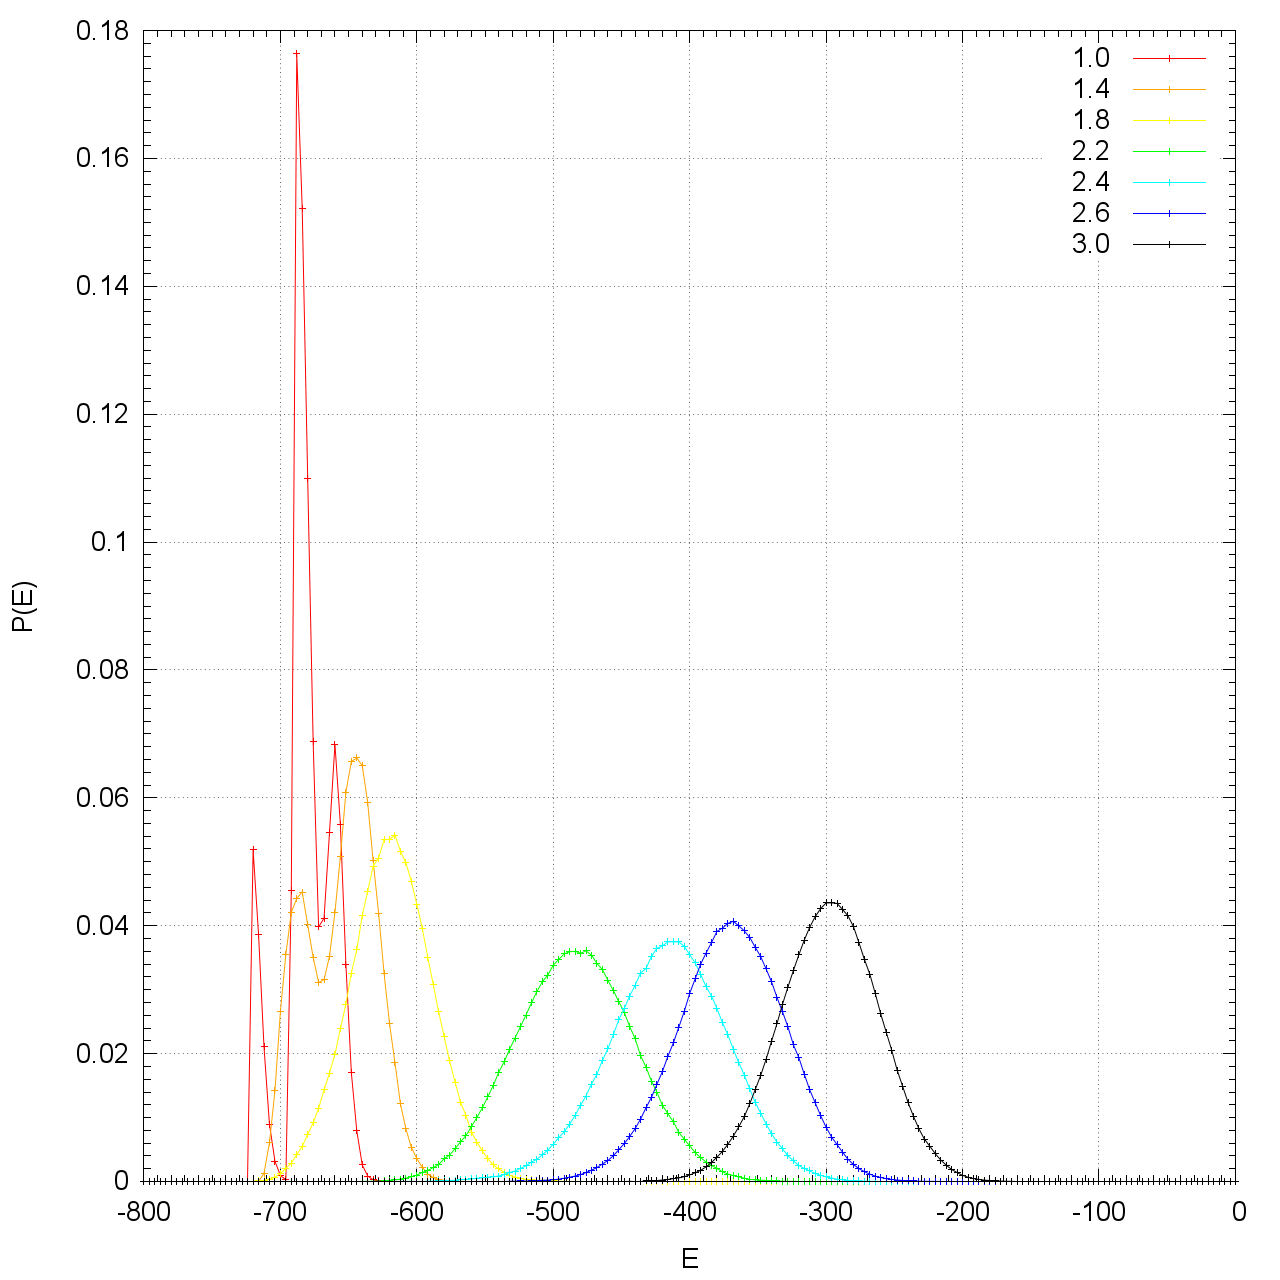
\includegraphics[width=.8\linewidth]{Energy_Countsr}
  \caption{{\footnotesize Random initial configuration}}
  \label{fig:sfig2}
\end{subfigure}
\caption{{\footnotesize Probability density function of the energy}}
\label{fig:fig}
\end{figure}
\end{center}
\noindent We have noticed that for low temperature the computed probabilities starting from the two configurations are very different. This is due to the fact that in this region of temperature the probability of accepting a flip is very low, as we can see from the plot; starting from the configuration with all the aligned spin is very unlikely to turn into more energetic configurations. Instead starting from a random matrix the system gets first a configuration made of blocks, more stable than the random one. At this point since accepting flip is unlikely the system oscillates only slightly around this configuration. Moreover while in the former case a flip is very energetically inconvenient (they are all variation of +8 J), in the latter one there are some possible flip corresponding to variations $\pm 4 J$. This can explain why in this case the probability is more spread over various energies 
than the previous one. 
\\
For higher temperatures the starting configuration does not affect significantly the final configuration and therefore the shape of the energy distribution, because the flip are much more likely (see figure 3).
\\
We have studied the behavior of the variances depending on the temperature. The value of the variances gets bigger until the region of the critical temperature, there it gets the biggest value and after that it starts decreasing as predicted from the theory.  
\begin{center}
\begin{tabular}[t]{|c|c|c|}
\hline
$K_b T [J]$ & $ \sigma^2_E random $ & $\sigma^2_E aligned$\\\hline
$1.0$ & 1.40563 & 0.03381\\\hline
$1.2$& 1.34009 &0.09960\\\hline
$1.4$ &  1.94504 &0.26172\\\hline
$1.6$ & 2.08009 &0.59659\\\hline
$1.8$&  2.93847 &1.21612\\\hline
$2.0$& 4.40327  &2.31210\\\hline
$2.2$& 6.06663  &4.20262\\\hline
$2.4$&5.20886& 6.22666\\\hline
$2.6$&  4.01864   &5.99270\\\hline
$2.8$& 4.26030 &4.97199\\\hline
$3.0$& 3.42241 & 4.32919\\\hline
\end{tabular}
\end{center}
The same discussion for the differences between the variances computed starting from different configuration at the same temperature still holds for this case. There is no need to plot the variance as we have already shown the plot of the heat capacity, which is the variance times some constants.
\section*{Bigger dimension matrices}
We have then applied our algorithm to bigger size matrices, respectively $40 \times 40$,$60 \times 60$, $80 \times 80$, $100 \times 100$, $150 \times 150$ and $200 \times 200$ matrices in order to make our model more and more realistic. For each case we have plotted the values of $E$, $\mathscr{M}$, $C_{V}$, $\chi$ for different values of the absolute temperature $\frac{k_{b}T}{J}$ in the range between 1 and 3, having picked data with a smaller step in the critic region around $T_{C}$. 
\\We decided not to run a fixed number of Monte Carlo cycles to compute the average with, but to scale this number with the total number of spins ($N^{2}$ where $N$ is the dimension of the matrix). In this way we have on average the same number of flipping attempts for each spin. We have chosen to run $10^{6}~N^{2}$ Monte Carlo cycles for each value of 
\\ To be sure to have a thermalized configuration, given the analysis made before, we decided to start collecting data after $50000\times N^2$ Monte Carlo cycles. 
\\The results are the following:
\begin{figure}[H]
\centering
\begin{subfigure}{.5\textwidth}
  \centering
  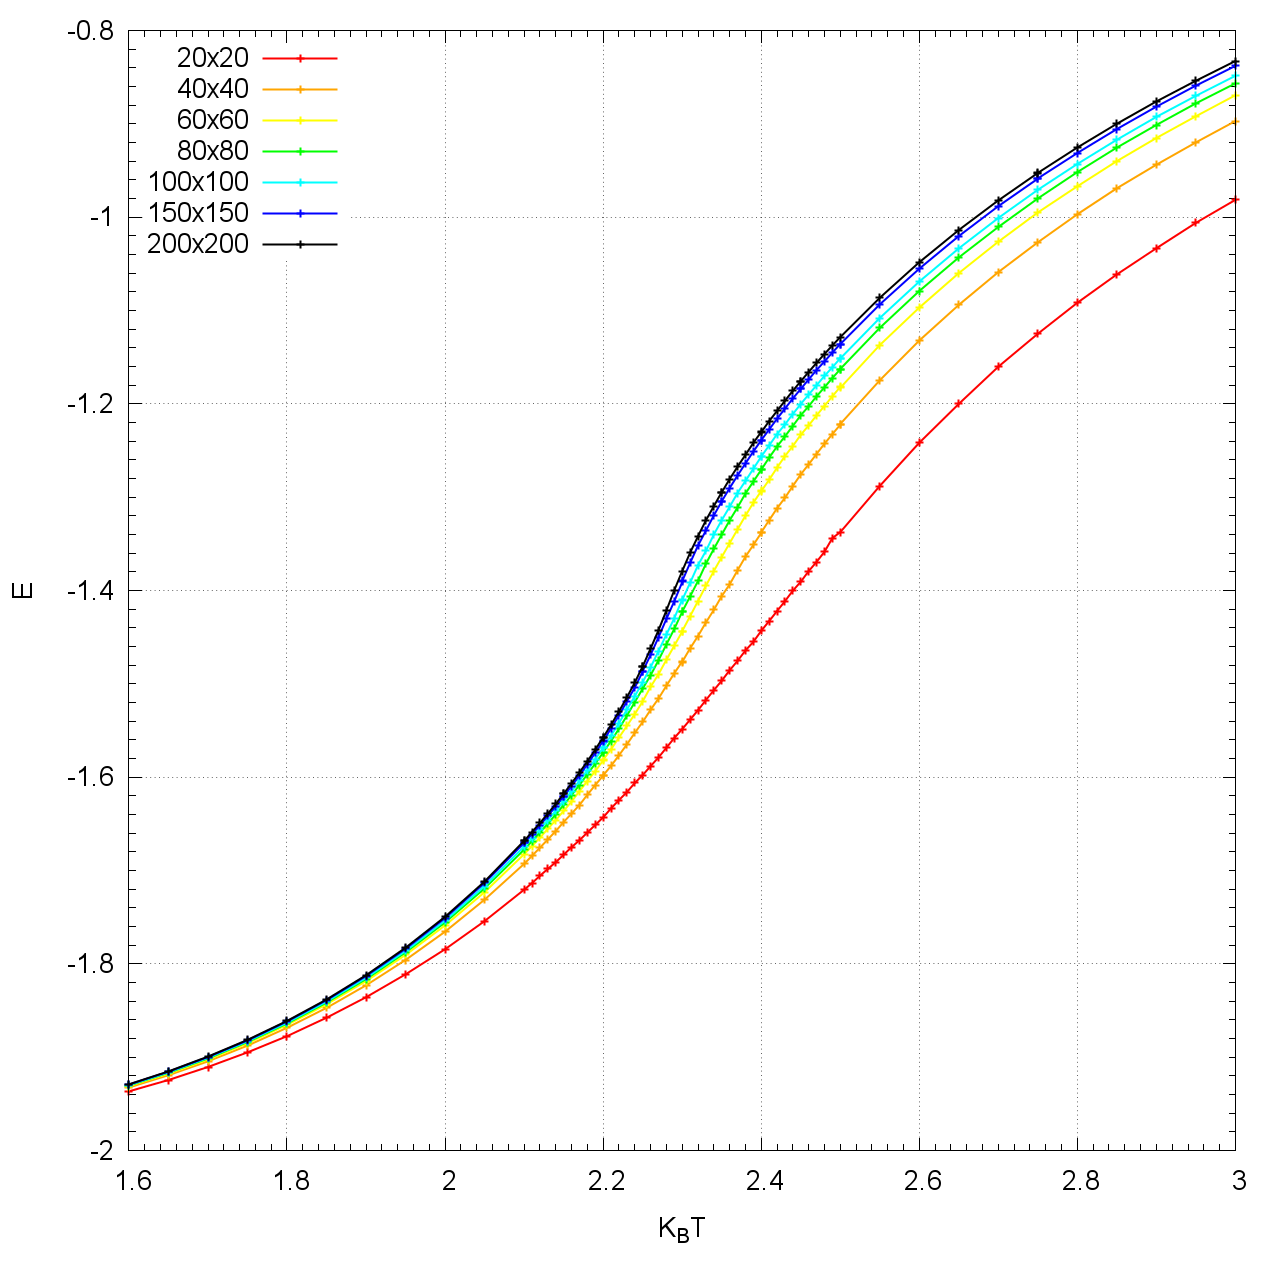
\includegraphics[width=1\linewidth]{Energy}
  \caption{{\footnotesize Energy}}
  \label{fig:sfig1}
\end{subfigure}%
\begin{subfigure}{.5\textwidth}
  \centering
  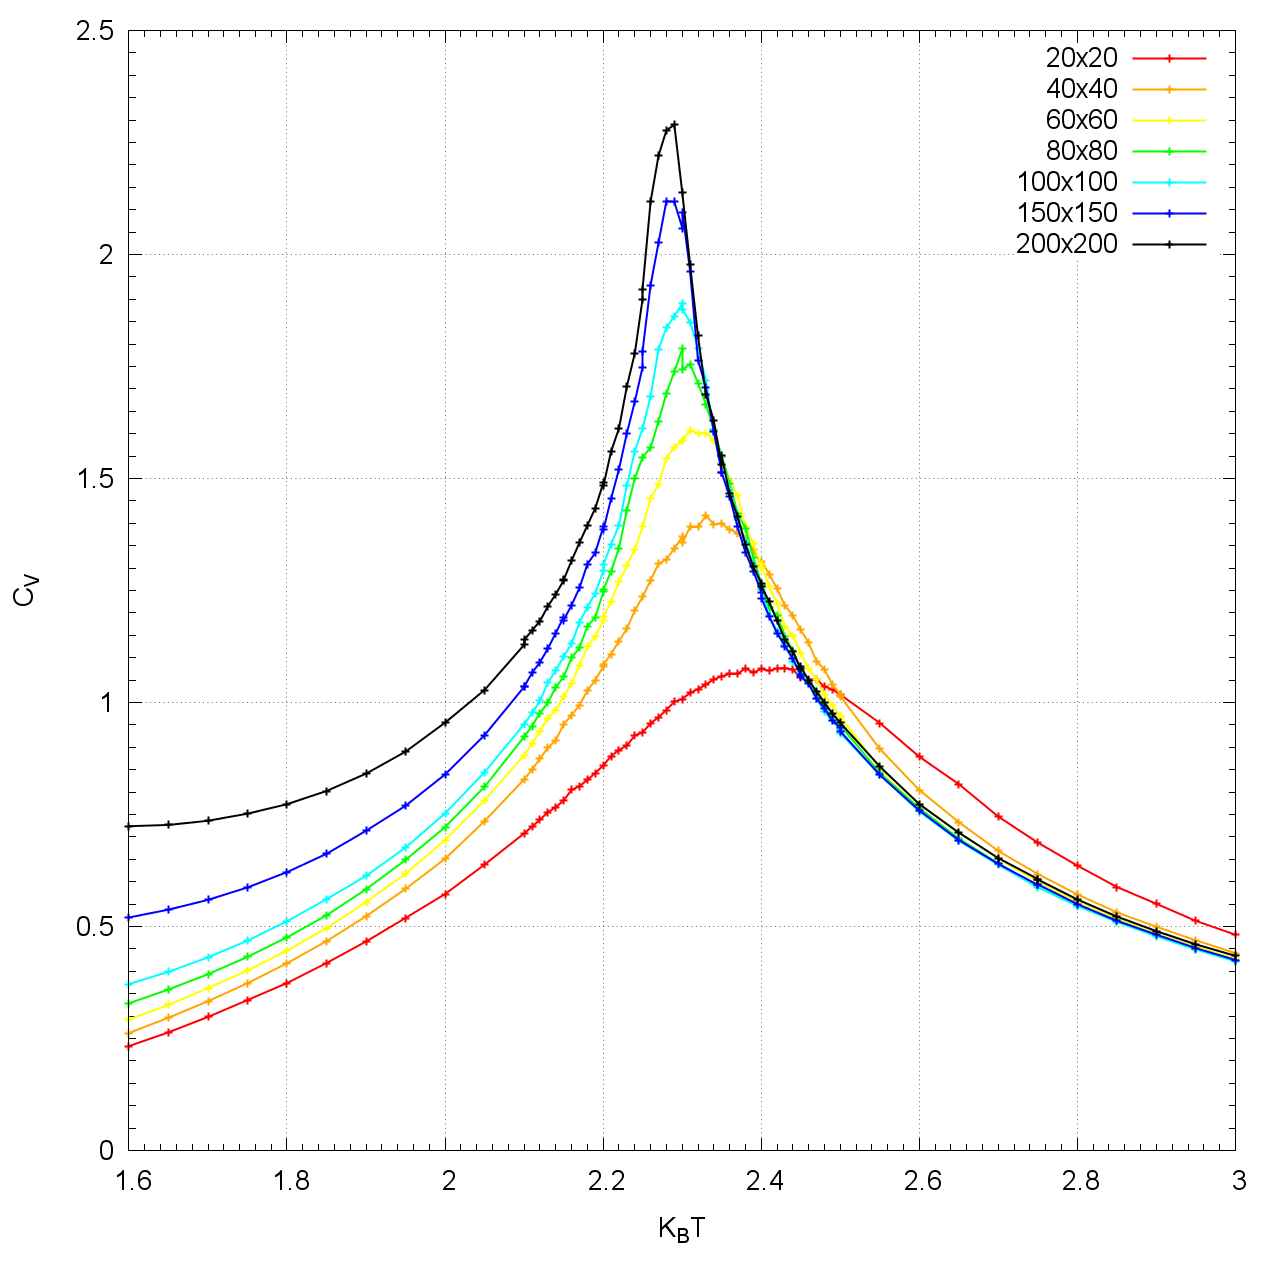
\includegraphics[width=1\linewidth]{Heat_Capacity}
  \caption{{\footnotesize Heat capacity}}
  \label{fig:sfig2}
\end{subfigure}
\end{figure}
\begin{figure}[H]
\centering
\begin{subfigure}{.48\textwidth}
  \centering
  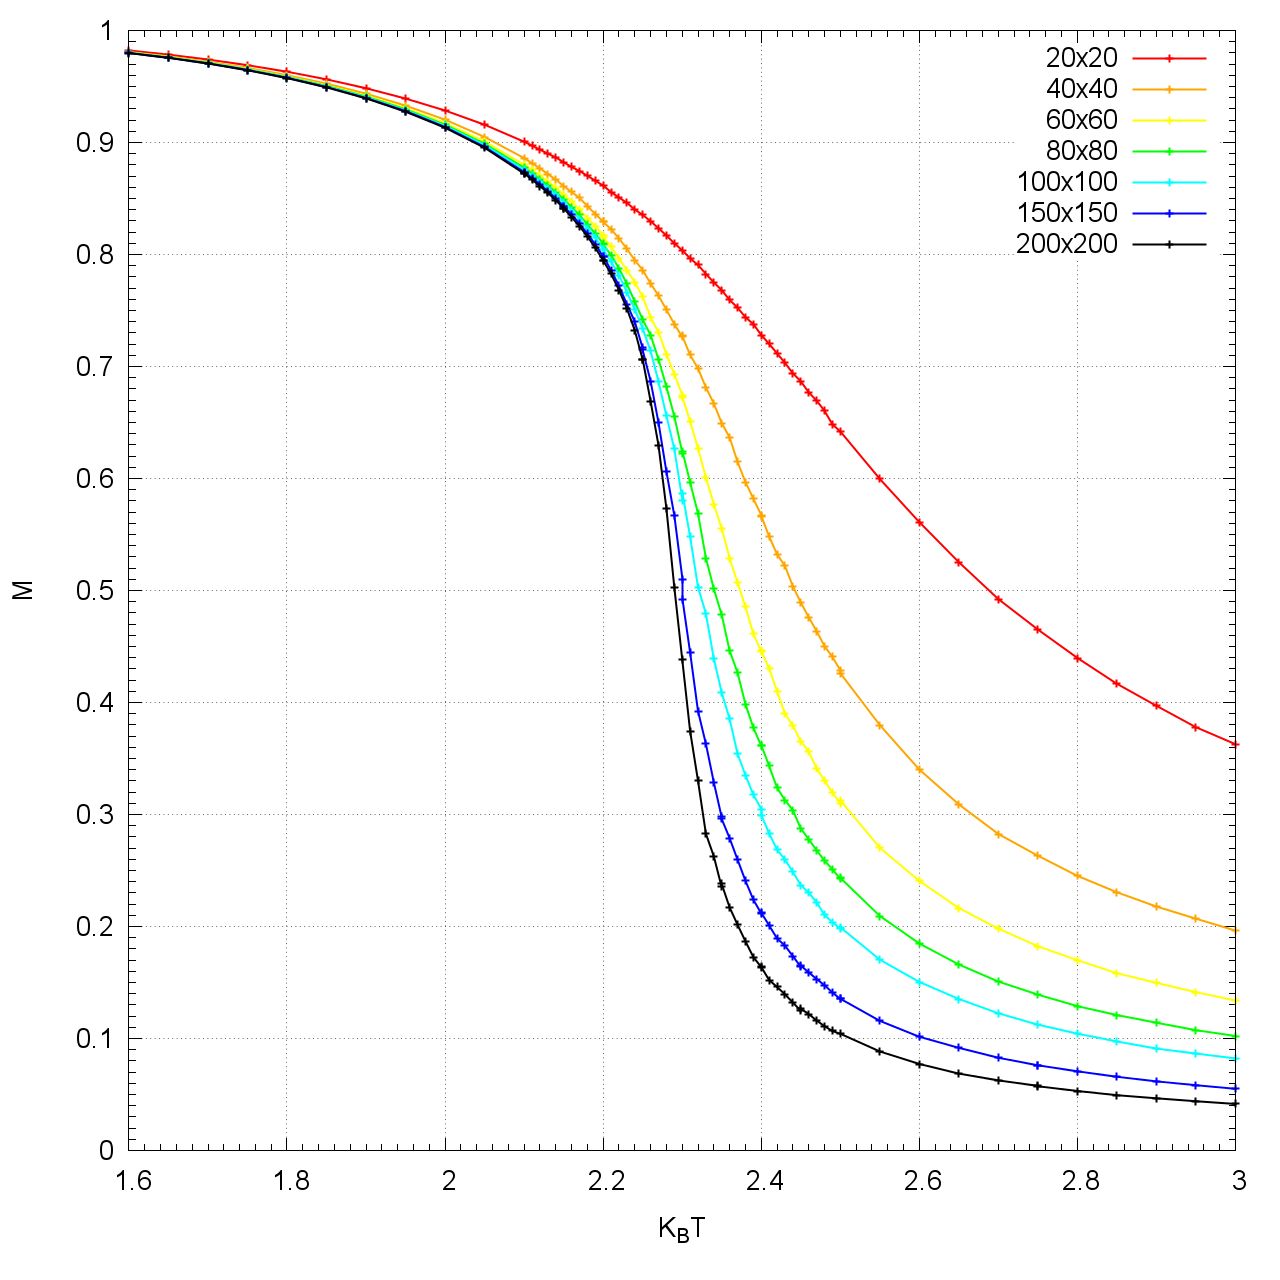
\includegraphics[width=1\linewidth]{Magnetization}
  \caption{{\footnotesize Magnetization}}
  \label{fig:sfig2}
\end{subfigure}
\begin{subfigure}{.48\textwidth}
  \centering
  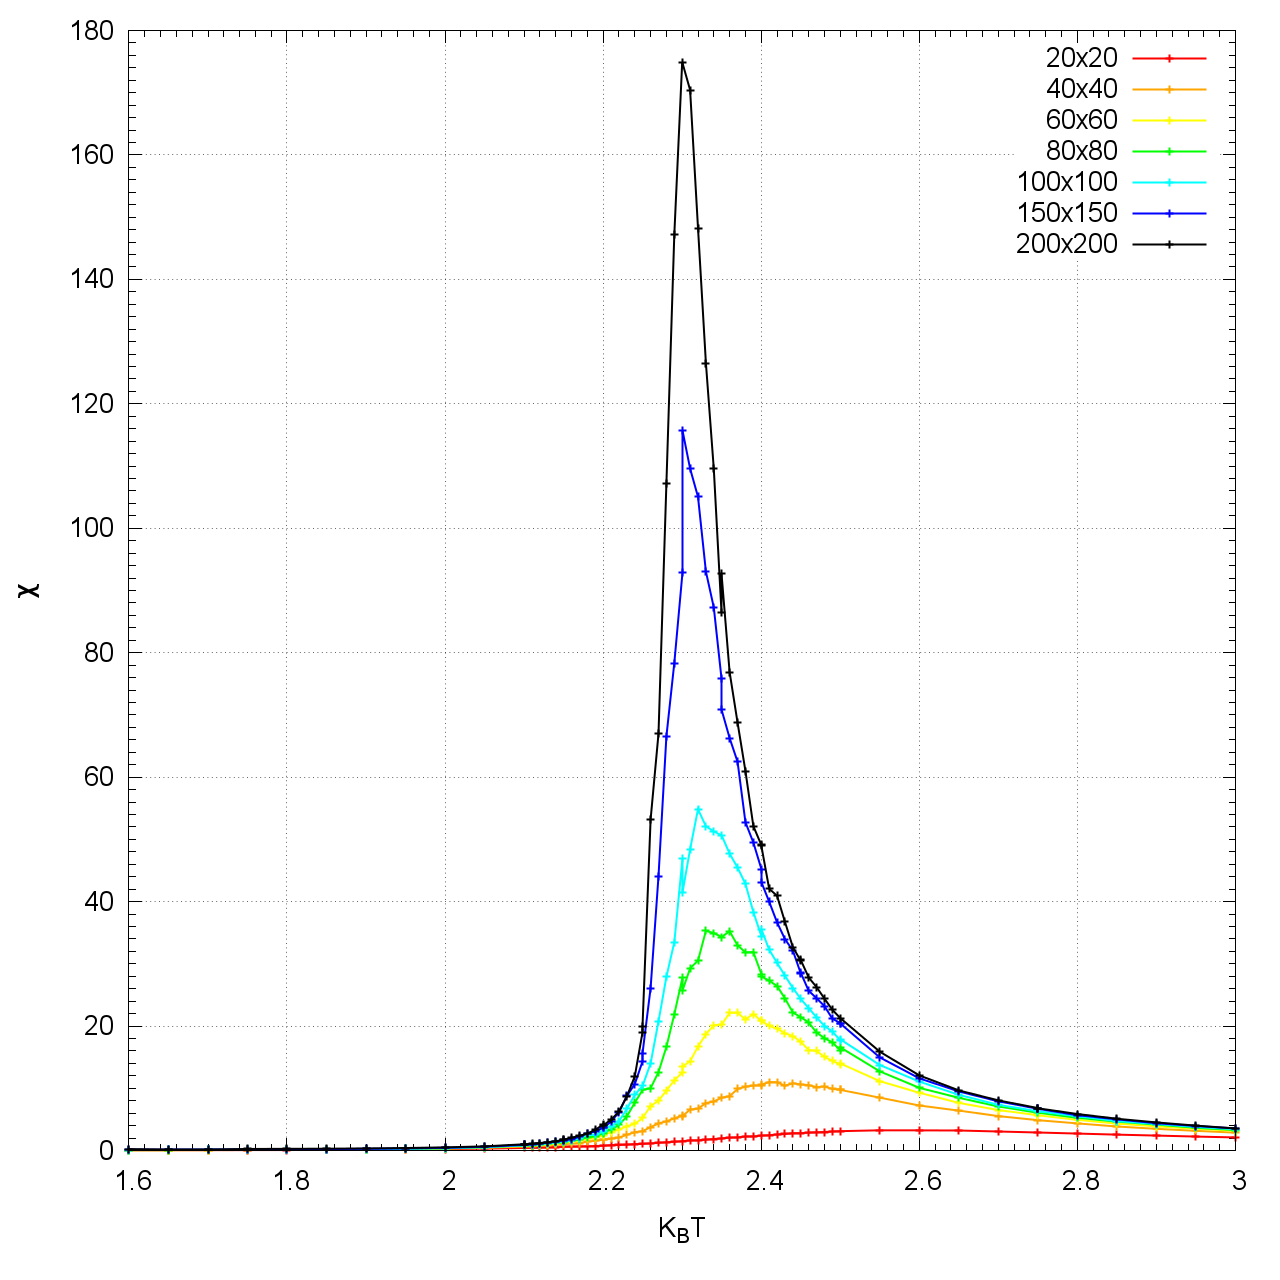
\includegraphics[width=1\linewidth]{Suscettibility}
  \caption{{\footnotesize Susceptibility}}
  \label{fig:sfig2}
\end{subfigure}
\caption{{\footnotesize Plots of the computed thermodynamic quantities for all the different matrix dimensions. Clear indications of a phase transition are the steep increase in the energy, the steep decrease of the absolute magnetization and the sharp peak in both the heat capacity and the susceptibility.}}
\label{fig:fig}
\end{figure}
\noindent Calculations carried on with bigger matrices resulted in more realistic results, especially for heat capacity and susceptibility, where the peak corresponding to the phase shift gets more sharp as the matrix size grows.
Moreover, referring to the graphs showing heat capacity (b) and susceptibility (d), it is clear that the estimate for $T_{C}$ (i.e. the value of $T$ for which these quantities have their maximum value) decreases as the size of the matrix grows, as expected according to eq. (12) and its value is roughly around the expected value $\sim 2.269$ but always bigger.
\\We have exploited the latter relation and our set of data to compute a more precise value for the critical temperature $T_{C}$ in the following section.
\paragraph{Estimate of $T_{C}$ for $L \rightarrow\infty$} We have exploited the relation $T_C(L)-T_C(\infty)=a L ^{-1/\nu}$, which link the critical temperature for a lattice with finite dimension $L$ and the critical temperature for an infinite lattice, to estimate this last quantity.
From the literature we know that $T_C(L=\infty) \simeq 2.269$.
\\
We know that $\nu=1$ and since we have already got thorough our algorithm the $T_C(L)$ for different size $L$, we have simply done a linear fit to extract $T_C(\infty)$. We have substituted $L^{-1}=x$ and we have done the linear fit $T_C(L)=a X + T_C(\infty)$ to extract the quantities $a$ and $T_C(\infty)$. 
\\
Since for the first two matrices ($20 \times 20$ and $40 \times 40$) the regions for which the curves of capacity and susceptibility have the maximum, so where the critical temperature should be located, are quite flat, we have preferred to not take into account their maximums.  In these cases they are more affected by random fluctuations than the others. 
\\
We have performed different fits for the critical temperatures got through the susceptibility and the ones for the heat capacity, because they result a little bit different. Anyway we have obtained both values in agreement within one $\sigma$ with the theoretical value and between each other. After these results we have done the last fit taking as critical temperatures the average between the ones from the susceptibility and the heat capacity, the result is still in agreement with the theoretical value.
Here the results:   \\
\begin{center}
\begin{tabular}{rl}
from the susceptibilities:& $T_{C}(L=\infty) =2.268 \pm 0.006  $\\
from the heat capacities: & $T_{C}(L=\infty) =2.274 \pm 0.007$  \\
from the average of  & \multirow{ 2}{*}{$T_{C}(L=\infty)=2.271 \pm 0.006   $}\\
the critical temperatures: & 
\end{tabular}
\end{center}
\newpage
\section*{Parallelization}
\noindent To keep the elapsed time as small as possible, we have implemented the parallelization of the code using $MPI$. Before the implementation however we used Valgrind to profile our code to optimize it before parallelizing since it is harder to profile code after implementing MPI.\\
This allowed us to perform 8 simultaneous Monte Carlo cycles, resulting in a much faster code. However  even with it just a computer was taking a lot of time doing all the operations. Especially the problem arose already with a $60 \times 60$ matrix, for which a calculation lasted 10 or more minutes. \\
For this reason we have adjusted the code segmenting the domain of temperature producing many executable programs for different domains. At this point we have run the different programs on different computers. Once got all the data we have merged them in a unique file. This allowed us to run the program using 96 processes in total (12 computers with 4 double thread cores) and to run the code for all matrix up to the size of $200 \times 200$ in approximately 1 hour of time in total (all 7 matrices). For the complete code of our programs look on \url{https://github.com/GioPede/FYS3150/tree/master/Project4}. There is also a simple animation of the cooling down of the system, which was an early version of our code, so it was parallelized using OpenMP instead.
\section*{Conclusions}
\noindent To sum up, Metropolis algorithm has proven to be a reliable simulation for a spin lattice experiencing a second order phase transition described by the Ising model, being more realistic as the size of the lattice increases. All physical quantities taken in account have varied as expected in relation to the temperature around $T_{C}$ and their behavior for larger matrices is fairly clear.  
\\We have also been able to estimate the value of the critical temperature for an infinite dimension lattice by a linear fit of its different (and more rough) estimates derived by the graphs of heat capacity and susceptibility for finite dimension matrices, resulting in a value which is compatible with the theoretical one. \\ 
We also achieved a fairly good optimization of the code using parallelization and we managed to run quite large simulations in reasonable time.
\\Finally, parallelization has proven to be necessary in order to run the algorithm for different temperatures for matrices bigger than $100 \times 100$ in a reasonable time.
\end{document}